\documentclass[a4paper,oneside,11pt]{article}
\usepackage{a4wide,graphicx,fancyhdr,amsmath,amssymb}

%-------- Macros and Definitions --------%

\setlength\headheight{20pt}
\addtolength\topmargin{-10pt}
\addtolength\footskip{20pt}

\newcommand{\subject}{2IO70 embedded systems}

\newcommand{\N}{\mathbb{N}}
\newcommand{\ch}{\mathcal{CH}}

\newcommand{\naam}{Reinhard Heinrich Bertram Vinzenz Freiherr von Pelden genannt Cloudt zu Lauersfort und Impel}

\fancypagestyle{plain}{%
\fancyhf{}
\fancyhead[LO,RE]{\sffamily\bfseries\large technische universiteit eindhoven}
\fancyhead[RO,LE]{\sffamily\bfseries\large \subject}
\fancyfoot[LO,RE]{\sffamily\bfseries\large department of mathematics and computer science}
\fancyfoot[RO,LE]{\sffamily\bfseries\thepage}
\renewcommand{\headrulewidth}{0pt}
\renewcommand{\footrulewidth}{0pt}
}

\pagestyle{fancy}
\fancyhf{}
\fancyhead[RO,LE]{\sffamily\bfseries\large technische universiteit eindhoven}
\fancyhead[LO,RE]{\sffamily\bfseries\large \subject}
\fancyfoot[LO,RE]{\sffamily\bfseries\large department of mathematics and computer science}
\fancyfoot[RO,LE]{\sffamily\bfseries\thepage}
\renewcommand{\headrulewidth}{1pt}
\renewcommand{\footrulewidth}{0pt}

\usepackage[margin=1in]{geometry}
\usepackage{float}
\usepackage{subcaption}
\usepackage{graphicx}

%-------- Title --------%

\title{\vspace{-\baselineskip}\sffamily\bfseries Machine Design}
\author{
	\makebox[.25\linewidth]{Sergio van Amerongen}\\0952200 \and
	\makebox[.25\linewidth]{Stefan Cloudt}\\0940775 \and
	\makebox[.25\linewidth]{Daan de Graaf}\\0956112 \and
	\makebox[.25\linewidth]{Robert van Lente}\\0953343 \and
	\makebox[.25\linewidth]{Tom Peters}\\0948730 \and
	\makebox[.25\linewidth]{Berrie Trippe}\\0948147 
	\and \makebox[.75\linewidth]{\textbf{Responsible:}} \and
	Robert van Lente\\ \tt{r.f.v.lente@student.tue.nl}
}
\date{\today}

%-------- Document --------%

\begin{document}
\maketitle

\section{Introduction}
We started our project by determining the features that we wanted to implement in our sorting machine, like user interaction and exception handling. These design decisions form the foundation of our mechanical machine design. The purpose of this document is to record the design decisions we made in the first stage of the project, from a mechanical point of view as well as
a user point of view.

\section{Design requirements}
In order to create a functioning sorting machine that can sort black and white discs, at least the following components are required.
\begin{itemize}
\item A container for storing unsorted discs
\item Two containers for storing the sorted discs
\item A sensor that can distinguish the different colour discs.
\item A transporter that is able to move the discs from the container to the sensor.
\item A transporter that is able to move the discs from the sensor to the appropriate container.
\end{itemize}

\section{Final Design}
The machine consists of a vertical tube in which the discs can be stored. A pin can be removed from the bottom of the tube, allowing the discs to fall on a platform below, one by one. A colour sensor is attached underneath this platform, such that it can detect the colour of the disc.
Next to this platform, a step motor is attached that rotates a wheel with three arms. These arms can push the disc of the platform, either on the left or the right side.
Below the platform, a seesaw is attached with both sides of the same length, such that the discs that fall on the platform can fall on these arms. A gyroscope is attached to the axis of this seesaw, such that rotations of the seesaw can be detected.
The discs then slide off the seesaw, allowing it to stabilize, and fall into one of two mountable trays.

\section{Design Decisions}
The machine went through several iterations before we settled on the final design. Below the decisions that we made during the design process are listed.

\subsection{Position of the colour sensor}
We had the option to attach the colour sensor in various ways to the machine. We chose to put it underneath the platform with the sensor pointing up, in such way that the arm of the motor could easily wipe the discs away.  Placing the sensor below the discs makes the sensor more reliable, since the surface of the discs on the bottom is larger than the surface on the side of the discs. It would also have been significantly more difficult to mount the colour sensor in a sideways or upright position because of the structural limitations of the construction set.

\subsection{Container}
The decision to use a tube-like structure was made early on, as it is the most compact way to store the discs. The vertical storage also has the added benefit of removing the need to create an additional transporter to move the discs from the container to the sensor, since a new disc will simply fall in place when the previous disc is moved away.

The height between the tube and the platform is designed to be slightly higher than the height of one disc. This ensures that only one disc will be moved from the tube at the time.

\subsection{Rotating arm}
The wheel to which the arms are attached are used to transport the discs from the sensor to the trays. We had options to put 3 or 4 arms on the wheel. We chose to go for 3 arms because then we would be able to attach a touch sensor which is used for calibration.

\subsection{Seesaw}
Initially, the plan was to use touch sensors to detect if a disc arrived in the correct tray. However, we quickly found that the discs did not weigh enough to trigger the touch sensors. Therefore we settled finally with the seesaw and a gyroscope attached to it.

\subsection{Trays}
We chose to use coffee cups for the trays in the machine, since these where readily and freely available. Other options would be buying plastic trays or building trays out of LEGO, which was not possible because there was not a sufficient number of parts in the construction set.

\begin{figure}[H]
\begin{subfigure}{0.5\textwidth}
	\centering
	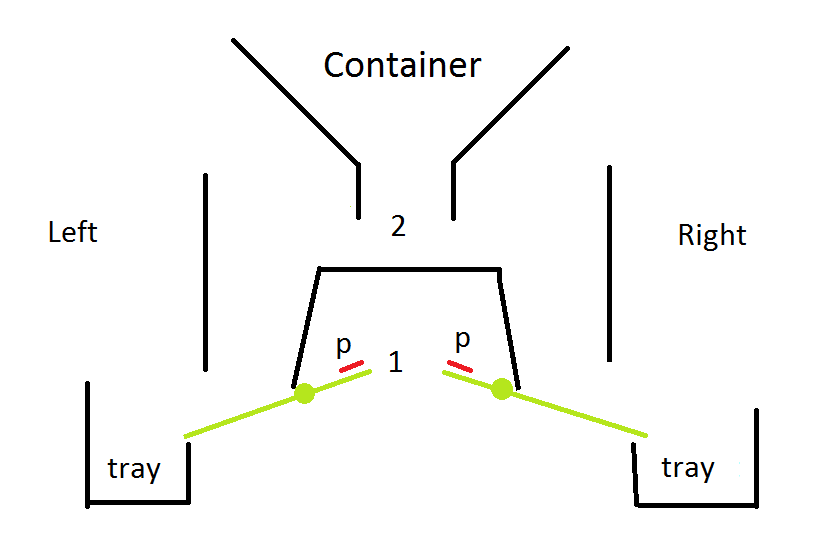
\includegraphics[width=80mm]{front}
	\caption{\label{firstfront}Front view}	
\end{subfigure}	
\begin{subfigure}{0.5\textwidth}
\centering
	\includegraphics[width=80mm]{top}
	\caption{\label{top}Top view.}
\end{subfigure}	
\caption{The initial design of the machine.}
\end{figure}

\begin{figure}[H]
	\centering
	\includegraphics[width=90mm]{frontnew}
	\caption{\label{front}The final front view of the machine.}
\end{figure}

\section{System Level Requirements}
\subsection{Use Cases}
The machine can be described as a finite automaton. This finite automaton is shown in figure
3. The machine has three buttons, which the user can utilize to control the machine. The
START/PAUSE button is used to start and pause the machine. The ABORT button is used to
stop the machine in case of emergency. The RESET button is used to reset the machine. The
user is required to add black or white discs to the container before starting the machine.
The machine, when finished without fatal error, produces two trays, one filled with white
and one filled with black discs. The machine will also display information about its current
state and progress on the display during the sorting process.

The sorting process is described by the following automaton. The initial state is the rest-
ing state. The user is required to prepare the machine as described in the User Constraints segment further in the document. None of the buttons should have any effect, except for the
START/PAUSE button. When this button is pressed, the machine should proceed to the
operating state.

In this state, the machine sorts the discs. Internally, it has a state in which it checks the
color of the disc, after which it moves to the correct sorting state in which it transports the disc
to the correct tray. If the RESET button is pressed in this state, the machine should return to
the resting state.

While in the operating state, if the START/PAUSE is pressed, the process should halt
and the machine should go into a paused state. When the START/PAUSE button is pressed
again, the machine should return to the operating state at the point where it was when the
START/PAUSE button was first pressed. If the RESET button is pressed in this pausing state,
the machine should return to the resting state.

While in the operating state, if the ABORT button is pressed or a fatal exception is encoun-
tered, the machine should immediately go into an exception state. In this state, the machine
must come to a full stop. The machine should only continue when the RESET button is pressed,
after which it returns to the resting state.

When the machine finds that there are no more discs left in the storage, it should go into a
finished state. Then, if the RESET button is pressed, the machine should return to the resting
State.

\begin{figure}[H]
	\centering
	\includegraphics[width=125mm]{machinedesign}
	\caption{\label{machinedesign}The finite state automaton of the machine.}
\end{figure}

\subsection{User Constraints}
\subsubsection{Machine Preparation}
Machine Preparation Before starting the operation of the machine with the START/PAUSE
button in the resting state, the user is expected to fill the disc storage device with black and
white colored discs that need to be sorted. Only discs are allowed in the disc storage and no
other objects should be placed in it. The user must also ensure that no discs are present in
other parts of the machine and that the disc trays are mounted to their mounting points prior
to starting execution. The disc trays should be empty. At most 12 discs may place into the
container. The user then has to proceed by starting the program. The tube can be filled with
discs after the machine has finished calibrating the moving arm.

After the machine has finished execution, the user will have access to two trays, one containing exclusively white discs, the other only contains black discs. When the machine indicates
that it has finished its sorting procedure, the user should remove the trays from their mounts
so he can dispose the discs somewhere else.

\subsubsection{Exceptions}
Possible errors are as follows:
\begin{figure}[H]
\centering
\begin{tabular}{|l|l|}
\hline
Error type & Fatal (= go to abort state)\\\hline
Disc does not reach the tray & Yes\\\hline
Disc arrives in the wrong tray & No\\\hline
Time to tray is higher than average & No\\\hline
Wrong input (i.e. different colour disc) & No\\\hline
Motor jams & Yes \\\hline
Gyroscope does not stabilise & Yes \\\hline
%Connection to peripheral lost & Yes \\\hline
Battery low & Yes \\\hline
Abort by user & Yes \\\hline
Software exception & Yes \\\hline
\end{tabular}
\end{figure}
When a disc does not reach the tray, the machine should stop, as there is may be an
obstruction in the path the disc takes from the sorting arm to the lever.

When a disc arrives in the wrong tray, the machine should stop, as something happened
that caused the disc to move to the wrong tray, even though the sorting arm tried to move
it to the correct tray. This means there must be a mechanical failure somewhere.

The Wrong Input error occurs when a disc is being detected with another color than white
or black. This could, for example, be a disc with the color red. This is not a fatal error because
we can specify an action that will be taken when this exception occurs. We may for example
want the machine to simply put the unknown disc in one of the trays anyway, say default the
destination to white, or we dispose all unknown discs into a separate tray.

%The connection to peripherals lost exception is marked as a fatal exception, because a defect
%in the controlling parts of the machine prevent it from functioning properly for obvious reasons.
%The user has to fix this by hand before the machine can be used again.

The machine will stop operation when the battery has less than 5% of charge left. This
is done to prevent the machine running out of power in between operations and ending in an
invalid state.

When an error occurs in the machine that is indicated with fatal, the user must remove all
discs from all parts of the machine. The user should then press the RESET button in order
to put the machine in its resting state. The user may then proceed to prepare the machine for
execution again, as described above, if desired.

\paragraph{Safety properties}
The machine should have the following safety properties. These are our
guarantees about the working and stopping conditions of the machine, in case something unex-
pected happens.

\begin{itemize}
	\item The ABORT button must stop all moving parts within 10 ms. This to make sure that the user is able to quickly stop the machine in case something can not be handled by the Machine.
	\item When the machine starts with discs loaded into the container, then the discs will be sorted
when it arrives in the finished state. The sorting process takes at most 5 minutes in the
default safe mode. However software specification may specify more modes.
	\item A fatal exception must stop all moving parts within 10 ms. This ensures that the machine
does not damage or even destroy itself when it is blocked in any way.
\end{itemize}

\section{Machine Interface}
\subsection{Lejos API}
The Lejos API provides access to buttons on the brick, sensors and actuators.
Buttons can be queried directly, but references to sensors and actuators must be instantiated
with a ’Port’ parameter indicating how they are connected to the brick. The following ports
are used in our design:

\begin{figure}[H]
\begin{tabular}{|l|l|}
\hline
\textbf{Peripheral} & \textbf{Port} \\
\hline
Colour sensor & Port 1 \\
Gyroscope & Port 2 \\
Touch sensor & Port 3 \\
Motor & Port A \\
\hline
\end{tabular}
\end{figure}

Motors expose methods that allow the developer to have to motor rotate an arbitrary number of degrees. Therefore, it is not necessary to implement pulse width modulation. One can call a method to fetch a sample from a sensor in the form of an array of floats. It is up to the developer to parse these in a meaningful way.

\subsection{Peripherals}

\subsubsection{Motor rotating arm}
This motor is connected to port A and rotates the arm which moves the discs. The arm has three legs with an angle of 120 degrees. The motor has basically three states: a resting state and two working states, one for every possible direction. The neutral position of the three legged arm is the position where the two arms closest to the place where the disc will land have an approximately identical distance to the disc. When the motor is in the resting state the three legged wheel has this neutral position. When the motor is in a working state the arms rotate left or right until the next neutral position of the wheel (120 degrees further), where it will transition to the resting state of the motor. During the working state the motor should not be jammed or obstructed in any way, or the motor will be jammed and trigger an exception.

When the motor is in a working state the arms rotate left or right until the next neutral position of the wheel (120 degrees further), where it will transition to the resting state of the motor. During the working state the motor should not be jammed or obstructed in any way, or the motor will be jammed and trigger an exception.

\subsubsection{Touch sensor calibrator}
The touch sensor, connected to port 3, is attached in such a way behind the sorting platform that the arms of the sorting wheel are able to fully press the sensor when it rotates. This way, it is possible to detect the position of the sorting wheel when it is rotating, which can be used to calibrate the sorting wheel through software.

\subsubsection{Gyroscope with seesaw}
To the seesaw a gyroscope is attached, which is wired to port 2. The seesaw has three states, a neutral state, a left-side down state and a right-side down state. The neutral state is the state in which the gyroscope when read returns a value indicating that it is in balance. The seesaw enters a left-side down state when a disc falls on the left side. The gyroscope will read a value indicating that it was unbalanced and that the left side went down.
This is analogous for the right side down state.

\subsubsection{Colour sensor}
The colour sensor, connected to port 1, gives a value indicating the colour of the surface above it. The colour sensor returns an integer indicating the colour of the disc (e.g. 0 for red, 1 for green etc.) currently on the platform, or -1 if only ambient light was reaches the detector, indicating that there is no disc on the platform. The sensor is able to distinguish 15 different colours, as shown in the following table:

\begin{figure}[H]
\begin{tabular}{|l|l|}
\hline
\textbf{Colour} & \textbf{Value} \\
\hline
None & -1 \\
Red & 0 \\
Green & 1 \\
Blue & 2 \\
Yellow & 3 \\
Magenta & 4 \\
Orange & 5 \\
White & 6 \\
Black & 7 \\
Pink & 8 \\
Gray & 9 \\
Light Gray & 10 \\
Dark Gray & 11 \\
Cyan & 12 \\
Brown & 13 \\
\hline
\end{tabular}
\end{figure}

\subsubsection{The brick}
The brick controls the sensors and actuators. The state of the buttons is either
up or down, which may be queried using the Lejos API. The buttons used are shown in figure \ref{brickbuttons}.
\begin{figure}[H]
	\centering
	\includegraphics[width=60mm]{BrickButtons}
	\caption{\label{brickbuttons}The buttons on the brick.}
\end{figure}

\section{Conclusion}
The design decisions recorded in this chapter will be built upon in the next phase of the
project, where we are going to specify the software specifications. The software specifications
are heavily dependent on the machine interface described in this chapter, since the machine
interface describe our assumptions about the machine API and the mechanical implementation.
The software specifications will describe how we are going to use this interface and how the
machine will behave.

\section{Sources}
\begin{description}
\item[Colour table]  http://www.lejos.org/ev3/docs/ - Constant Field Values
\end{description}
\end{document}
